\cotefile{12}
\scanpage{150}
Considérons un foncteur additif
\diagram{\begin{tikzcd}
\mathcal V \arrow[rr,"H"] \arrow[dr,"\uline h"'] && \mathcal C \\
& \mathcal M \arrow[ur,"T"'] &
\end{tikzcd}}
\margin{$C$ cat. abélienne}
comment exprimer que $T$ est \uline{fidèle} ?

Comme $T$ est exact, il revient au même de dire que
\[
\deleted{\unsure{T\text{ f.}}}\quad
\left\{\begin{array}{l}
T\text{ fidèle}\\
T(M)=0\ \Longrightarrow\ M=0\\
T\text{ conservatif}\\
T:\operatorname{End}(M,M)\xrightarrow{\deleted{\unsure{\simeq}}}\operatorname{End}(TM,TM)\quad\text{injectif}
\end{array}\right.
\]
\deleted{Cela s'exprime aussi par la propriété}

\uline{Pour ceci il f. et s. que $\unsure{M|H}$ soit fidèle}

\figure{\begin{tikzpicture}[x=1cm,y=1cm]\draw (0,0) .. controls (4,.02) and (7,.65) .. (10,.7);\end{tikzpicture}}

\uline{Exemple}\qquad $k$ corps alg. clos.
\diagram{\begin{tikzcd}[column sep=small]
\mathcal V_0 \arrow[d] & \text{catégorie des schémas projectifs lisses sur }k\\
\mathcal V & \text{catégorie ayant \unsure{mêmes} objets que }\mathcal V_0,\ \text{mais}
\end{tikzcd}}
les morphismes sont
\[
\operatorname{Fl}(X,Y)=\unsure{\bigoplus|\prod}_{i,j} C^{m_j}(X_i\times Y_j)
\]
où les $X_i$ sont les comp. conn. de $X$, les $Y_j$ celles de $Y$, $\dim Y_j=m_j$ ; $C^q(Z)$ désigne les classes de cycles\inserted{ à coeff en $\mathbf Q$,} mod $\mathbf Q_\ell$-homologie, de codim $q$ sur $Z$. La composition se fait suivant
\mspage{149}

\scanpage{151}
la composition connue des classes de correspondance.
\inserted{On a catégorie additive (objet nul est $\varnothing$, somme est $\amalg$).}

Si on admet que l'équiv. hom. $=$ équiv. numérique, alors on déduit (par th. de finitude de la cohomologie) que les $\operatorname{Fl}(X,Y)$ sont des \unsure{esp.} vectoriels de dim finie sur $\mathbf Q$ ; si on admet l'inégalité de Hodge, \unsure{un|les} $\operatorname{Fl}(X,X)$ devient une algèbre involutive du type de \unsure{Castelnuovo}-Weil.... donc est semi-simple. D'où une catégorie \deleted{de} $\mathcal M$, mais on \unsure{va} considérer celle associée à $\mathcal V^\circ$, de sorte que on a un foncteur \uline{contravariant} additif universel
\diagram{\begin{tikzcd}
\mathcal V^\circ \arrow[r,dash,"\uline h"] & \mathcal M
\end{tikzcd}}

D'ailleurs, on a un foncteur évident
\[
H^{*}(,\mathbf Q_\ell):\mathcal V^\circ\longrightarrow\operatorname{Mod}_{\mathrm{t.f.}}(\mathbf Q_\ell)
\]
en associant à tout $X\in\operatorname{Ob}\mathcal V$ le module $H^{*}(X,\mathbf Q_\ell)$. Ce foncteur est \uline{fidèle}, par définition \unsure{même} des $\operatorname{Hom}$ dans $\mathcal V$ ($+$ dualité ...).

On trouve un foncteur exact fidèle \unsure{can.}
\[
T_\ell:\mathcal M\unsure{\mathbin{-}|\longrightarrow}\operatorname{Mod}_{\mathrm{t.f.}}(\mathbf Q_\ell)
\]
appelé \uline{foncteur de Tate}.
\mspage{150}

\scanpage{152}
Autres foncteurs canoniques sur $\mathcal M$ : foncteurs de Hodge, de \deleted{\unsure{Hodge}} De Rham (fidèles en car. $0$), de Betti (si $k=\mathbf C$)\deleted{\unsure{k}}. Il y a d'ailleurs des structures supplémentaires importantes à mettre sur ces foncteurs....

On a un bifoncteur
\diagram{\begin{tikzcd}
\mathcal V\times\mathcal V \arrow[r,dash] & \mathcal V\\
X,Y \arrow[r,rightsquigarrow] & X\times Y
\end{tikzcd}}
qui est associatif et commutatif, d'où une structure \unsure{multiplication|multiplicative} dans $\mathcal M$.
La formule de Künneth en cohomologie implique que $T_\ell$ est un foncteur qui commute \deleted{aux} à l'opération $\otimes$, donc aux opérations tensorielles.

\figure{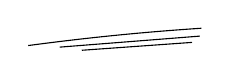
\begin{tikzpicture}[x=1cm,y=1cm]
\draw (0,0) .. controls (0.9,0.12) and (1.6,0.18) .. (2.2,0.22);
\draw (0.4,-0.02) -- (2.18,0.12);
\draw (0.68,-0.06) -- (2.08,0.04);
\end{tikzpicture}}

Revenons à la situation abstraite précédente. Nous supposons maintenant que pour tout $X\in\operatorname{Ob}\mathcal V$, on se donne des \inserted{\uline{projecteurs}} $\pi_i\in\operatorname{Fl}(X,X)$ $(i\in\mathbf N)$, \inserted{presque tous nuls,} de somme $1$, deux à deux orthogonaux, fonctoriels en
\mspage{151}

\scanpage{153}
$X$. En d'autres termes, on suppose donné \deleted{un hom d'anneaux topologiques}\inserted{ des \deleted{\unsure{hom}} éléments}
\[
\pi_i\in\operatorname{End}\operatorname{id}_{\mathcal V},\quad\text{avec}\quad
\pi_i^2=\pi_i,\quad\pi_i\pi_j=\pi_j\pi_i=0\quad\text{si }i\ne j,
\]
\[
\deleted{k[[\pi_1,\ldots,\pi_n,\ldots]]/(\pi_i^2-\pi_i,\ \pi_i\pi_j,\ \deleted{\unsure{\pi_j}}\ \sum\pi_i-1}
\]
et $\sum\pi_i=1$. \margin{somme infinie !}
Alors les $\pi_i$ s'étendent à $\mathcal M$, qui devient une catégorie graduée, \deleted{\unsure{par}} ``somme'' de catégories $\mathcal M^{i}_{\deleted{\unsure{i}}}$, dont les objets sont appelés ``motifs\inserted{ effectifs} de poids $i$''.

On suppose de plus que dans $X\boxtimes Y$, on a
\[
\pi_n(X\boxtimes Y)=\sum_{i+j=n}\pi_i(X)\boxtimes\pi_j(Y);
\]
celà implique alors que
\diagram{\begin{tikzcd}
\mathcal M^i\times\mathcal M^j \arrow[r,dash] & \mathcal M^{i+j}
\end{tikzcd}}
par l'accouplement $\otimes$, et fournit donc un lien étroit entre les $\mathcal M^i$. Ainsi, le groupe\inserted{ de classes} $K$ de $\mathcal M$ est un \uline{$\lambda$-anneau gradué}.
\margin{L'objet unité $\Lambda(0)$ est de degré $0$. \uline{On va supposer que c'est le seul objet simple de ce degré}, et \uline{que \unsure{son end. soit} \inserted{\unsure{identifié à}} $\mathbf Q$}.}

\deleted{\unsure{On}} Je suppose maintenant fixé, de plus, un objet \deleted{\unsure{Z(1)}} $\Lambda(-1)$ de $\mathcal M$,\inserted{ de degré $\unsure{\rho|\beta}\geq1$,} tel que, posant \deleted{\unsure{\Lambda}} $M(1)=M\otimes\Lambda(1)$, \deleted{\unsure{le foncteur}} le
\mspage{152}

\scanpage{154}
foncteur $M\mapsto M(-1)$ \uline{soit pleinement fidèle}.
Ses itérés sont les $M\mapsto M(-n)=M\otimes\Lambda(-n)$, $\Lambda(-n)\simeq\Lambda(\unsure{1|-1})^{\otimes n}$.
Noter que
\[
\operatorname{Hom}(\Lambda(-n),\Lambda(-n))\simeq\operatorname{Hom}(\Lambda(0),\Lambda(0))\simeq\mathbf Q
\]
On introduit alors formellement aussi les $M(n)$, $n\in\mathbf Z$, en considérant la catégorie pseudo-$\varinjlim$ des copies de $\mathcal M$, par les foncteurs $M(-1)$. Ainsi tout objet de la nouvelle catégorie $\widetilde{\mathcal M}$ \deleted{``motifs \unsure{virtuels}\inserted{\deleted{\unsure{effectifs}}}''} s'écrit
\[
M(i)\qquad i\in\mathbf Z,\quad M\in\operatorname{Ob}\mathcal M,\quad\text{avec}
\]
\[
\operatorname{Hom}(M(i),N(j))\simeq\operatorname{Hom}(M(i+r),N(j+r))
\]
où $r$ est pris tel que $i+r,j+r\leq0$, alors $M(i+r)$, $N(j+r)$ ont déjà un sens.
\margin{$\Lambda(1)$ de degré $-\rho$}
La catégorie $\widetilde{\mathcal M}$ est encore graduée (de $-\infty$ à $+\infty$ maintenant) périodique de période $\rho$ par le foncteur \deleted{\unsure{M}} $M\mapsto M(-1)$. En dim $i\geq0$ (\unsure{cas auquel} on se \unsure{ramène}) elle s'écrit comme
\[
\operatorname{Ps}\varinjlim_k\mathcal M^{i+k\rho},
\]
où
\diagram{\begin{tikzcd}
\mathcal M^{i+k\rho}\arrow[r] & \mathcal M^{i+(k+1)\rho}
\end{tikzcd}}
est le foncteur pl. fd $M\mapsto M(-1)$.
\margin{\uline{N.B.} Un sous motif d'un motif effectif est effectif..}
\mspage{153}

\scanpage{155}
\deleted{Décomposition canonique}

\uline{Niveau d'un motif}

\unsure{a)} \uline{Motif effectif} $M$ de degré $i\geq0$ est dit de niveau $\leq i-k\rho$ s'il est isomorphe à un motif de la forme $M'(\unsure{k|-k})$, où $M'$ est un motif effectif de degré $i-k\rho$.
Les motifs effectifs, de degré $i\geq0$ fixé, de niveau $\leq i-k\rho$ font une sous-catégorie \uline{épaisse} de $\mathcal M^i$, donc tout objet\inserted{ $M$} de $\mathcal M^i$ se décompose canoniquement en une somme d'un\inserted{ tel} objet maximal $M'$ de niveau $\leq i-k\rho$, et d'un \inserted{autre sous-}objet. \deleted{\unsure{M}}
Ainsi,
\[
\mathcal M^i\simeq\mathcal P^i\times\mathcal P^{i-\rho}(\unsure{-1|1})\times\mathcal P^{i-2\rho}(\unsure{-2|2})\times\cdots,
\]
\margin{projections $\kappa_{i,k}$}
où $\mathcal P^j$ désigne la catégorie des motifs effectifs de degré $j$ \deleted{primitifs} dont aucun sous-motif\inserted{ $\ne0$} n'est de niveau $\leq j-\rho$.
\margin{motifs \uline{primitifs de niveau $j$}}

Celà donne donc une décomposition de $\mathcal M^{*}=\mathcal M$ en termes des $\mathcal P^i$ (pour les structures additives). La structure \unsure{multiplication|multiplicative} est connue quand on connaît les foncteurs
\diagram{\begin{tikzcd}
\unsure{\theta|\Theta}^{i,j,k}:\mathcal P^i\times\mathcal P^j\arrow[r] & \mathcal P^{i+j-k\rho}
\end{tikzcd}}
\margin{$\unsure{\theta|\Theta}^{ijk}(M,N)=\deleted{\unsure{\kappa(M\otimes N(-}}\kappa_{i,k}(M\otimes N)(k)$.}

b) Niveau d'un motif quelconque (pas néc. effectif).
Se définit en se ramenant au cas précédent....
\mspage{154}

\scanpage{156}
\uline{\unsure{Duals|Duels} et Homs de motifs}

On suppose que\inserted{ $\rho=2$ et que} pour tout motif effectif $M$, de degré $i\geq0$, $\mathcal Hom(M,\Lambda(-i))$ existe\inserted{ et est un motif eff.} (où $\mathcal Hom(M,N)$ est défini axiomatiquement par
\[
\operatorname{Hom}(P,\mathcal Hom(M,N))\simeq\operatorname{Hom}(P\otimes M,N)
\]
On constate que si $M,N$ sont des motifs effectifs de degrés $i,j$, tels que $\mathcal Hom(M,N)$ existe, alors $\mathcal Hom(M,N)$ est de degré $j-i$. Ici, posant
\[
M^{*}=\mathcal Hom(M,\Lambda(-i))\qquad\deg M=i
\]
on trouve que $\deg M^{*}=\deg M$. On trouve d'ailleurs que si $\mathcal Hom(M,N)$ existe dans $\mathcal M$, il existe aussi dans $\widehat{\mathcal M}$ et est le même.

On voit que pour \unsure{tt|$\forall$} $M$ de degré $i$, et \unsure{tt|$\forall$} $N$, $\mathcal Hom(M,N(-i))$ existe, car on aura
\[
\mathcal Hom(M,N(-i))\simeq M^{\unsure{*|\circ}}\otimes N
\]
(vérification facile). \deleted{D'où} Cela prouve que pour tout $N$ (pas néc. \unsure{hom.})
\mspage{155}

\scanpage{157}
$\mathcal Hom(M,N(\unsure{-j|j}))$ existe pour $j$ grand, dans la catégorie des motifs effectifs. Enfin, $\mathcal Hom(M,N)$ existe dans la catégorie de tous les motifs, comme on voit en prenant $\mathcal Hom(M,N(\unsure{j|-j}))(-j)$. On arrive ainsi à construire $\mathcal Hom(M,N)$ pour $M,N\in\operatorname{Ob}\widehat{\mathcal M}$ quelconques, avec les règles de calcul évidentes. On définit aussi $\check M=\mathcal Hom(M,\Lambda(0))$, et on trouve $\mathcal Hom(M,N)\simeq\check M\otimes N$. Mais on fera attention que si $M$ est effectif, $\check M$ ne l'est que si $\deg M=0$.

\[
B(M,N)\simeq\operatorname{Hom}(M\otimes N,\Lambda(-i))\simeq\operatorname{Hom}(M,N^{*})\simeq\operatorname{Hom}(N,M^{*})
\]
``formes bilinéaires'', avec $M,N$ de degré $i$.
Si $M=N$, on a la notion de forme alternée, forme symétrique.
\margin{\uline{N.B.} Forme non dégénérée en $M$ :}
\[
M\mathbin{-}N^{*}\quad\text{mono.}\quad\Longleftrightarrow\quad N\longrightarrow M^{*}\text{ est }\deleted{\text{injectif}}\inserted{\text{\unsure{épim.}}}
\]
On définit de même forme non dégénérée en $N$.

\margin{?}
Si $M=N$, les deux notions sont équivalentes car \deleted{tout hom} pour un hom $M\longrightarrow M^{*}$, dire que c'est \unsure{mono} ou \unsure{épimorphe} \deleted{\unsure{ou}} \unsure{un isom.} est pareil.
\mspage{156}

\scanpage{158}
\uline{Involutions.} Supposons $\alpha\in B(M,M)$ forme \deleted{\unsure{quelconque}} \deleted{\unsure{et}} non dégénérée, et sym. ou \deleted{anti} alternée, alors \deleted{Alors par} \unsure{l'iso} $\widetilde\alpha:M\simeq M^{*}$. Soit de même $\beta\in B(N,N)$ d'où $\widetilde\beta:N\longrightarrow N^{*}$ $(M,N\text{ de deg }i)$.
Soit $u:M\mathbin{-}N$, on définit alors $u':N\mathbin{-}M$ par comm. du diagramme ci-contre.
\diagram{\begin{tikzcd}
M \arrow[r,leftarrow,"u^{\prime\deleted{\unsure{*}}}"] \arrow[r,phantom,"\deleted{\unsure{\rightarrow}}"{description,pos=.88,inner sep=0pt}] \arrow[d,"\widetilde\alpha"'] & N \arrow[d,"\widetilde\beta"]\\
M^{*} & N^{*} \arrow[l,"\unsure{{}^tu^{*}|u^{*}}"']
\end{tikzcd}}
\margin{transposé}
On trouve les relations habituelles
\[
\begin{aligned}
(u\pm v)'&=u'\pm v'\\
(uv)'&=v'u'\\
1'&=1\\
(u')'&=u
\end{aligned}
\]
\margin{si $\alpha$ et $\beta$ sont tous deux \deleted{\unsure{sym.}} \inserted{sym.} ou tous deux alternés.}
En particulier sur $\operatorname{End}(M)$ on a une structure d'algèbre involutive sur $\mathbf Q$. \deleted{\unsure{Alors}}
Si $\alpha$ est remplacé par $\alpha_1$, $\beta$ par $\beta_1$, on aura
\[
\widetilde\alpha_1=\widetilde\alpha\circ A,\qquad\widetilde\beta_1=\widetilde\beta\circ B\qquad(A\in\operatorname{End}(M),\ B\in\operatorname{End}(N))
\]
et la nouvelle ``adjonction'' sera
\[
u''=\deleted{\unsure{\widetilde\beta_1}}\ \widetilde\alpha_1^{-1}\circ u^{*}\circ\widetilde\beta_1
=A^{-1}\widetilde\alpha^{-1}u^{*}\widetilde\beta B\qquad\text{i.e}
\]
\[
u''=A^{-1}u'B
\]
En particulier, si $M=N$, on a dans $A$ une involution définie mod \deleted{\unsure{autom. intérieurs}}\inserted{\unsure{transformation} de $u\mapsto u'$ en} $u\mapsto A^{-1}u'A$, où $A$ est un élément autoadjoint (?)
\mspage{157}

\scanpage{159}
\uuline{Formes définies positives sur les motifs}

Ceci implique déjà que les $\operatorname{End}(h^i(X))$ sont des \uline{algèbres de Riemann}, et par suite $\frac12$ simples, (ce qui permet de construire la catégorie des des motifs comme catégorie \uline{abélienne}).

De plus, cette catégorie des motifs $\mathcal M$, et sa complétée $\widetilde{\mathcal M}$, \unsure{recevra} d'importantes structures suppl.

Discutons d'abord le degré d'indétermination possible du système $\varphi_X$. Pour ceci, \unsure{notons} \deleted{pour} regardons ce qui se passe si on remplace les $(\varphi_i)$ par $(\varepsilon_i\varphi_i)$ ($\varepsilon_i$, \uline{signes} ne dépendant que de $i$). Les axiomes (i) et (iii) restent vérifiés, mais (ii) seulement si on a $\varepsilon_i\varepsilon_j=\varepsilon_{\unsure{i+j|ij}}$, donc $\varepsilon_i$ doit \deleted{être de la forme $\unsure{(\pm1)}$} $+1$ pour tt $i$, \uline{ou} $\unsure{(-1)^i|\varepsilon^i}$ --- il est caractérisé en se donnant ce qu'il doit être en degré $1$.
On imposera, dans le cas de la géom. alg., qu'il corresponde aux formes de polarisation sur les V.A.
\mspage{158}

\scanpage{160}
\mspage{159}

VII.19

\uline{Proof:} We will show that $A$ satisfies the hypothesis of
Theorem VII.12, namely, that $A$ is a local unique factorization
domain and that every separable extension is a unique factorization
domain. We know that $A$ is a unique factorization domain (as we
remarked in Lemma VII.16). In Lemma VII.14 we saw that every
separable extension is a semi-local regular domain, and in Lemma
VII.16 that every semi-local regular domain is a unique factorization
domain. Thus by Corollary VII.13 $\mathcal B(A)\subset\mathcal B(K)$.

THEOREM VII.18. If $A$ is a regular domain, then
$\mathcal B(A)\unsure{\subset|\subseteq}\mathcal B(K)$.

\uline{Proof:} $A$ is integrally closed, since $A_{\uline M}$ is integrally closed
for each maximal ideal $\uline M$ and $A$ is the intersection of the $A_{\uline M}$.
We will show that $A$ has the property that every reflexive ideal is
projective, and that every finitely generated reflexive module whose
endomorphism ring is projective is itself projective. Then, applying
Theorem VII.8, $\mathcal B(A)$ is contained in $\mathcal B(K)$.

Let $\unsure{\mathfrak a|a}$ be a reflexive ideal of $A$. Then, since $A_{\uline M}$ is a unique
factorization domain for every maximal ideal $\uline M$ of $A$, $\mathfrak a_{\uline M}$ is a
principal ideal of $A_{\uline M}$, and thus free. Therefore $\mathfrak a$ is projective
over $A$.

Now suppose $M$ is a finitely generated reflexive module over $A$
such that $\operatorname{Hom}_A(M,M)$ is projective. Then $M_{\uline M}$ is reflexive as an

\scanpage{161}
Supposons que pour tout $X\in\mathcal V$, \inserted{on ait un}
$(\uline h(X)=(\uline h^i(X)))$
\deleted{\unsure{soit muni d'un}}
un ensemble $\Phi_X$ de formes fondamentales
$\{\varphi\}$, chaque $\varphi=(\varphi_i)$,
$\varphi_i\in\operatorname{Hom}(\uline h^i(X)\otimes\uline h^i(X),
\Lambda(-i))$, de façon que les conditions suivantes
soient vérifiées :

(i) Si $\varphi\in\Phi_X$, $\psi\in\Phi_Y$, alors
$\varphi\oplus\psi\in\Phi_{X\amalg Y}$.

(ii) Si $\varphi\in\Phi_X$, $\psi\in\Phi_Y$,
\deleted{et $u:X\longrightarrow Y$, d'où
$h(u):\uline h^i(Y)\longrightarrow\uline h^i(X)$, \unsure{pourrions}}
alors $\varphi\otimes\psi\in\Phi_{X\unsure{\boxtimes|\otimes}Y}$

$(\mathrm{iii}_0)$ Sur
\deleted{$\varphi\in\Phi_X$, alors $\varphi(0)$ sur $\unsure{X|\overline X}=e$, donc
$\uline h^0(e)\unsure{\otimes|\simeq}\uline h^0(e)\simeq Q$, \unsure{tous}}
\inserted{$h^0(X)$, \unsure{considéré de} \unsure{dim} finie sur $Q$, les $\varphi\in\Phi_X$ sont}
des formes \uline{définies positives}
\margin{[il suffit $X=e$ \deleted{\unsure{lorsque}}]}

\unsure{Sans doute on le supprimera} \unsure{par}
\deleted{(iii)}

(iii) Si $\varphi\in\Phi_X$, $\psi\in\Phi_Y$,
$u:X\mathbin{-}Y$ d'où
$u^{(i)}:h^i(\unsure{Y|X})\mathbin{-}h^i(Y)$,
\unsure{prenant} $\unsure{\delta|s}u^{(i)}:h^i(Y)\mathbin{-}h^i(X)$,
[\unsure{relativ.}: $\varphi,\psi$], on a
\[
\boxed{\operatorname{Tr}(\unsure{\delta|s}u^{(i)}u^i)\geq0,
\quad\text{égalité ssi }u^{(i)}=0}
\]
\mspage{160}

\scanpage{162}
\mspage{161}
VII.20

as an $A_{\uline M}$-module, and
$\operatorname{Hom}_{A_{\uline M}}(M_{\uline M},M_{\uline M})$ is projective as an
$A_{\uline M}$-module for every maximal ideal $\uline M$ of $A$. Now $A_{\uline M}$ has the
property that every reflexive ideal is projective, and we know from
Theorem VII.17 that $\mathcal B(A_{\uline M})\subset\mathcal B(K)$ for every maximal ideal $\uline M$
of $A$. Thus, from Theorem VII.8, $M_{\uline M}$ is projective as an
$A_{\uline M}$-module for each $\uline M$. Therefore $M$ is a projective $A$-module,
and so $\mathcal B(A)\subset\mathcal B(K)$.

Radcliffe Institute for Independent Study

Wellesley College

\scanpage{163}
On va exprimer l'axiome (iii) de façon équivalente,
en introduisant $\chi=\varphi\otimes\psi$ sur $X\boxtimes Y$.
\inserted{et tordant $\Lambda(i)$.}
On trouve alors
\deleted{sur $\operatorname{Hom}(\Lambda(-i),H^{2i}(X\boxtimes Y))$}
la forme

(iii bis) \uline{Sur} \deleted{$\unsure{H^{2i}(X)(i)|H^i(X)(i)}$}
$\operatorname{Hom}(\Lambda(-i),\unsure{\uline H^{\unsure{2|2i}}|\uline h^{2i}}(X))
\simeq\Gamma\uline h^{2i}(X)(i)$,
\uline{la forme induite par la forme} $\varphi_i$ est \uline{définie positive}.

\margin{L'équivalence de (iii) avec (iii bis) vaut moyennant (ii) et le
cas évident $(\mathrm{iii}_0)$, \unsure{utiliser} \uline{dualité} pour
exprimer les homomorphismes $X\mathbin{-}Y$ en termes d'éléments de
$\Gamma H^{2i}(X\boxtimes Y)(i)$}

Prenons $\varphi,\psi\in\Phi_X$,
\inserted{avec \deleted{$\unsure{\varphi(x,y)}$} $\widetilde\psi=\widetilde\varphi\circ A$}
Alors pour tt $u:X\longrightarrow X$, induisant
$u=u^{(i)}:\uline h^i(X)\mathbin{-}\uline h^i(X)$,
\deleted{on a \unsure{un transp.} $\unsure{u}$}
Soit $u'$ le transposé de celui-ci relatif à $\varphi,\varphi$,
alors le transposé relatif à $\varphi,\psi$ est $u''=u'A$,
et on en conclut $\operatorname{Tr}uu''\geq0$ donc $\operatorname{Tr}uu'A\geq0$.
\uline{Cela exige que} $A$ \uline{est dans le cône positif}
de l'algèbre \deleted{involutive} de Riemann
$\operatorname{End}(\uline h^i(X))$ définie par $\varphi$, --- ce qui
revient à $=$, $\varphi$ et $\psi$ sont des formes
``équivalentes'' du \unsure{pt} de vue des structures
Riemanniennes qu'elles définissent.
\mspage{162}

\scanpage{164}
\mspage{163}
VII.18

LEMMA VII.15. If $S$ is a semi-local domain and $S_{\uline M}$ is
a unique factorization domain for each maximal ideal $\uline M$ of $S$,
then $S$ is a unique factorization domain.

\uline{Proof:} Let $\unsure{\mathfrak p|\mathcal P}$ be a prime ideal in $S$. We will show that $\mathfrak p$ is
a principal ideal. Since $S$ is an integrally closed domain, this is
equivalent to saying that $S$ is a unique factorization domain. If $\uline M$
is a maximal ideal in $S$, $\mathfrak p_{\uline M}$ is either $S_{\uline M}$ or a prime ideal in $S_{\uline M}$.
Since $S_{\uline M}$ is presumed to be a unique factorization domain $\mathfrak p_{\uline M}$ is
a principal ideal (in either case). Thus $\mathfrak p_{\uline M}$ is a free $S_{\uline M}$ module
for each $\uline M$, and $\mathfrak p$ is therefore projective when considered an
$S$-module. Then the Remark in [4, p. 377] proves that $\mathfrak p$ is a
principal ideal in $S$.

LEMMA VII.16. Every regular semi-local domain is a unique
factorization domain.

\uline{Proof:} If $S$ is a regular semi-local domain, then $S_{\uline M}$ is a
regular local domain for each maximal ideal $\uline M$ of $S$. Auslander
and Buchsbaum have shown in [3] that every regular local domain is a
unique factorization domain.

THEOREM VII.17. If $A$ is a regular local domain, then
$\mathcal B(A)\subset\mathcal B(K)$.

\scanpage{165}
\deleted{\unsure{Soit maintenant}} \inserted{Plus gén\textsuperscript{t} soit}
$M$ un motif effectif, \unsure{hom} de degré $i$.
Choisissons un hom \uline{injectif} $M\longrightarrow\uline h^i(X)$
et considérons la forme induite par une $\varphi\in\Phi_X$, soit $\varphi_0$.
Choisissant de $=$ $M\longrightarrow\uline h^i(Y)$, et $\psi\in\Phi_Y$,
d'où $\psi_0$. Je dis que $\varphi_0$ et $\psi_0$ sont
\inserted{\uline{définies}} et \uline{équivalentes}.
\deleted{ce qui signifie que $\operatorname{Tr}$}
La première p\textsuperscript{té} résulte des
\deleted{\unsure{propriétés}} \deleted{\unsure{le fait que} $\varphi$ est définie}
\deleted{\unsure{les}} \deleted{positive}\ldots Riemanniennes\ldots
La deuxième \deleted{\unsure{reste}}

\diagram{\begin{tikzcd}[column sep=small,row sep=large]
\substack{\uline h^i(X)\\ \varphi}
  \arrow[dr,"\lambda"]
  \arrow[dr,bend right=35,"{\deleted{\unsure{\varphi|\psi}}\lambda'}"']
& & & \substack{\uline h^{\unsure{j|i}}(Y)\\ \psi}
  \arrow[dl,"\mu"'] \arrow[dl,bend left=35,"\mu'"]\\
& \substack{M\\ \varphi_0}\arrow[r,"u"] & \substack{M\\ \psi_0} &
\end{tikzcd}}

exprime que la forme $\operatorname{Tr}(u'u)$ est définie,
\inserted{$u\in\operatorname{End}(M)$}
où $u'$ est définie par $\varphi_0$ et $\psi_0$. Or
\deleted{\unsure{car}} pour cel, il suffit de
\deleted{\unsure{prouver}} \inserted{noter} que la forme
\[
\operatorname{Tr}(\mu u\lambda')'(\mu u\lambda')
=\operatorname{Tr}\lambda u'\mu'\mu u\lambda'
=\operatorname{Tr}\lambda'\lambda u'\mu'\mu u
\]
l'est, or $\mu'\mu=\mathrm{id}$,
\inserted{$\lambda'\lambda=\mathrm{id}$}
donc cette forme est $\operatorname{Tr}u'u$, OK !
On pourra donc, \uline{sur un motif effectif}, définir une classe
d'équivalence de formes riemanniennes, \unsure{soit}
$\unsure{\Phi_M|\Psi_M}$ (\uline{\unsure{ens.} saturé !}). Les $\Psi_M$ satisfont
\mspage{164}

\scanpage{166}
\mspage{165}
VII.17

elements in a minimal basis of $\uline M$ is equal to the dimension of $R$.

A noetherian domain $R$ is said to be a \uline{regular domain} if and
only if $R_{\unsure{\mathfrak p|\mathcal P}}$ is a regular local domain for every prime ideal $\mathfrak p$ of $R$.
(A necessary and sufficient condition that $R$ be a regular domain is
that $R_{\uline M}$ be a regular local domain for every maximal ideal $\uline M$). If
$R$ is a regular domain $R=\bigcap_{\{\uline M\}}R_{\uline M}$ where $\{\uline M\}$ is the set of
maximal ideals of $R$.

A \uline{semi-local ring} is a noetherian ring with a finite number of
maximal ideals.

We will sketch the proofs of the following lemmas, which are
well-known facts in the theory of local rings.

LEMMA VII.14. If $R$ is a regular local domain and $S$ is an
unramified extension, then $S$ is a semi-local regular domain.

\uline{Proof:} Since $S$ is unramified over $R$, $S$ is regular, by a
special case of [2, Corollary 5.2]. Furthermore, any finite
extension of a local domain is semi-local. We see this by considering
$R/\uline M\otimes_R S=S/\uline M S$ where $\uline M$ is the maximal ideal of $R$. $S/\uline M S$ is
finitely generated over the field $R/\uline M$ and therefore has but a finite
number of maximal ideals. But the maximal ideals of $S$ are in one-
to-one correspondence with the maximal ideals of $S/\uline M S$. Thus $S$
is semi-local.

\scanpage{167}
Les conditions \deleted{\unsure{aussi}} analogues à (i), (ii), (iii)
$(\mathrm{iii}_0)$ \margin{$(\mathrm{iii}_0)\longrightarrow\text{normalisation}$}.

\deleted{Lorsqu'on dispose du \unsure{supplément} de structure
\unsure{exprimé} par un $\Lambda(-1)$,}
On a un iso
\[
B(M(-1),M(-1))\simeq B(M,M)
\]
et il y a lieu de vérifier la condition que $\Psi_{M(-1)}$ correspond à
$\Psi_M$. Ça ne doit pouvoir faire de difficulté.
\deleted{Pour l'expliciter en termes de $\mathcal V$ directement,
il faudrait expliciter comment \unsure{on obtient} $\Lambda(-1)$
en termes d'un objet.}
En fait, utilisant la propriété (ii), on trouve qu'il suffit de vérifier que
la forme canonique $1$ sur
\[
1\in B(\unsure{M|\Lambda}(-1),\Lambda(-1))
\]
est dans $\Psi_{\Lambda(-1)}$.
\deleted{Ça ne saurait} La vérification dans le cas de Géométrie Alg. est triviale.

Ceci permet d'étendre la notion de forme \inserted{\uline{définie}}
positive aux motifs non nécessairement effectifs.
\mspage{166}

\scanpage{168}
\mspage{167}
VII.15

which has the property that every separable extension is a unique
factorization domain, then every finitely generated reflexive module
over $A$ which has a projective endomorphism ring is itself projective.

\uline{Proof:} Let $M$ be a finitely generated reflexive module over $A$
such that $\operatorname{Hom}_A(M,M)$ is projective. Suppose $M\neq0$. We know
from Theorem III.4 and Theorem VI.9 that $\operatorname{Hom}_A(M,M)$ is
separable at minimal primes and therefore, since it is projective,
it is separable over $A$ [4, Proposition 4.6]. Then, by Lemma VII.10
we know that there is a splitting ring $S$ for $\operatorname{Hom}_A(M,M)$ such that
$S$ is a finitely generated unramified extension of $A$ and an integrally
closed noetherian domain. Under the hypothesis, $S$ is a unique
factorization domain.

Now we have $\{\operatorname{Hom}_A(M,M)\otimes_A S\}=\{S\}$ in $\mathcal B(S)$. But
$\operatorname{Hom}_A(M,M)\otimes_A S\approx\operatorname{Hom}_S(M\otimes_A S,M\otimes_A S)$ [7, p. 124, Ex.11] so
$\{\operatorname{Hom}_S(M\otimes_A S,M\otimes_A S)\}=\{S\}$ in $\mathcal B(S)$. Thus
$\operatorname{Hom}_S(M\otimes_A S,M\otimes_A S)\approx\operatorname{Hom}_S(V,V)$
where $V$ is a finitely generated faithful projective
module over $S$ [4, Proposition 5.3]. Then from [9, Lemma 9] we
see that there is a finitely generated projective $S$-module $J$ of rank 1
such that $M\otimes_A S\approx V\otimes_S J$. Thus $M\otimes_A S$ is a projective $S$-module.
Since $S$ is a projective $A$-module, $M\otimes_A S$ is a projective $A$-module.
Now a finitely generated module over a noetherian ring $A$ is pro-
jective if and only if it is free over $A_{\uline M}$ when localized at every

\cotefile{15}
\scanpage{2}
\unsure{Groupe|Groupes} de Galois \unsure{motivique|motiviques}
commutatif

Cas d'un corps de
base fini

\scanpage{3}
\uline{Catégorie des motifs sur $\mathbf F_p=k$}

$\mathcal M$ admet un foncteur fibre $T_\ell$ sur $Q_\ell$ (à valeurs en dans $\operatorname{Mod}(\widehat{\mathbf Z},Q_\ell)$) pour tt $\ell\ne p$.
Pour $\ell=p$, il y a un foncteur $T_p$ sur $Q_p$, cohomologie cristalline (foncteur à valeurs dans \deleted{$\operatorname{Mod}($}$F$-cristaux sur $Q_p$, donc dans vectoriels sur $Q_p$ munis d'un autom., donc dans $\operatorname{Mod}(\mathbf Z,Q_p)$ --- Attention, ici on ne peut remplacer $\mathbf Z$ par $\widehat{\mathbf Z}$ !]

Soit \deleted{$\unsure{\mathcal M}$} $\operatorname{Niv}^0(\mathcal M)$ la sous-catégorie des motifs de niveau $0$
\[
\operatorname{Niv}^0(\mathcal M)^0\qquad\rule{6cm}{0.3pt}\quad\rule{0.7cm}{0.3pt},\ \text{poids zéro.}
\]
Il y a un foncteur fibre naturel \deleted{\unsure{indépendant}} \inserted{intrinsèque} en $Q$ sur la sous-catégorie $\operatorname{Niv}^0(\mathcal M)^0$, soit
\diagram{\begin{tikzcd}
F^0:\operatorname{Niv}^0(\mathcal M)^0 \arrow[rr] \arrow[dr] && \operatorname{Mod}(Q,\deleted{\widehat{\mathbf Z}}) \\
& \operatorname{Mod}(Q,\widehat{\mathbf Z}) \arrow[ur] &
\end{tikzcd}}
\margin{\unsure{équivalent} aux faisceaux de $Q$-(\unsure{vect.}\ \unsure{dim. finies}) sur $k$}
\margin{\unsure{valable} pour tout $k$}
défini par
\[
F^0(H^*(X))=f_*(\uline{Q}_X)
\]
si $X$ fini sur \deleted{$k$} --- cela définit $F^0$ sur $\operatorname{Niv}^0(\mathcal M)^0$
\[
F^0(Q(1))=Q.
\]
Donc la gerbe \inserted{$\mathcal G$} des foncteurs fibres de $\mathcal M$ contient la sous-gerbe \inserted{\deleted{$\unsure{\mathcal G}$}$\unsure{\mathcal H}$} des foncteurs fibres de $\mathcal M$ prolongeant $F^0$, laquelle correspond (si $G$ est le lien de $\mathcal M$, qui est \inserted{\unsure{un}} un groupe \uline{commutatif} sur $k$, si on admet les \unsure{p\textsuperscript{tés}} de \unsure{densité|dualité}....) au groupe
\[
H=\operatorname{Ker}(G^0\xrightarrow{\unsure{\epsilon|e}}G_m)
\]
Par ailleurs, \deleted{\unsure{si on admet}} en vertu des conj. de Tate et de Tate-Honda, $G$ est le groupe de \unsure{t. m.} sur $Q$, dont le groupe des caractères $\Gamma$ est
\mspage{2}

\scanpage{4}
163.

Proofs are omitted. As in (ii) of Theorem 25.1, they are computational (though somewhat more involved, especially for characteristic two).
\[
*\qquad\qquad *\qquad\qquad *
\]
REMARK 25.3. Let $R$ be a two-dimensional normal local ring with maximal ideal $m$. We assume, for simplicity, that $R/m$ has characteristic $\ne2$. Without any further assumption on $R/m$, we have actually show that $R$ has a rational singularity, a trivial group $H$, and the configuration diagram (k) (cf. earlier part of \S24) \uline{if and only if} $R$ satisfies (ii) of Theorem 25.1 (cf. also Remark 25.2).

The other types of rational singular points with trivial group $H$ can be discussed similarly. The results are given below. Once again proofs are computational and are omitted.
\diagram{\begin{array}{ll}
\text{\uline{Configuration}}&\text{\uline{Relation on suitable}}\\
\text{\uline{Diagram}}&\text{\uline{generators}}\quad x,y,z\quad\text{\uline{of}}\quad m.\\[1em]
\text{\unsure{1-3|l-3}}&z^2+ax^3+bx^2y+cxy^2+dy^3=0\\
&(a,b,c,d\in R,\ \text{and if }\bar a,\bar b,\bar c,\bar d\\
&\text{are the respective residues mod. }m,\\
&\text{the form}\\
&\bar aX^3+\bar bX^2Y+\bar cXY^2+\bar dY^3\\
&\text{is irreducible over }R/m).
\end{array}}
\mspage{3}

\scanpage{5}
le sous groupe
\[
\Gamma\subset\overline Q^*
\]
formé des $\lambda$ tels que l'on ait
\[
\left\{\begin{array}{l}
\lambda\unsure{\in}\ \text{entiers algébriques}\\
\lambda\ \text{une unité }\ell\text{-adique pour }\ell\ne p\\
|\lambda_i|=p^{\nu/2}\ \text{pour }\deleted{\unsure{\exists}}\ \nu\in\mathbf Z^+\ \text{convenable,}\\
\qquad\text{pour tt conjugué de }\lambda_i
\end{array}\right.
\]
Le groupe $G^0$ est défini par
\[
\Gamma/\Gamma_{\mathrm{tors}}=\Gamma/(\text{racines de l'unité})
\]
L'hom $G\overset{\unsure{\epsilon}}{\unsure{\mathbin{-}|\longrightarrow}}G_m$ correspond à l'hom
\diagram{\begin{tikzcd}
\mathbf Z \arrow[r] & \Gamma\\
1\arrow[r] & p
\end{tikzcd}}
et $\operatorname{Ker}(\epsilon|G^0)=\operatorname{Ker}(G^0-G_m)$ est défini par le groupe de caractères
\[
\Gamma/\{\text{racines de l'unité},p^\nu\}=\Gamma'
\]
qui est un groupe \deleted{\unsure{ent.}} dont le sous groupe de torsion est $\simeq\mathbf Z/2\mathbf Z$
\diagram{\begin{tikzcd}
\unsure{0}\arrow[r] & \mathbf Z/2\mathbf Z\arrow[r] & \Gamma'\arrow[r] & \Gamma'/\operatorname{tors}(\Gamma')\arrow[r] & 0\\
&1\arrow[r,mapsto]&\begin{array}{c}\text{classe de}\\p^{1/2}\text{ dans }\Gamma'\end{array}&&
\end{tikzcd}}
On a donc
\diagram{\begin{tikzcd}
\unsure{0}\arrow[r]&H^0\arrow[r]&H\arrow[r]&\mu_2\arrow[r]&0
\end{tikzcd}}
et $H^0$ est un \uline{\unsure{tor. compact}}. En fait, l'hom $i:G_m-G$ définit $i|\mu_2:\mu_2\longrightarrow H^0$, et donne un \uline{splitting}
\[
H\simeq H^0\times\mu_2
\]
\mspage{4}

\scanpage{6}
162.

\uline{Characteristic} 5
\[
\alpha z^2+\beta y^3+x^5=\gamma x^4
\]
where $\gamma$ is one of
\diagram{\begin{array}{ll}(a)&0\\(b)&y\end{array}}

\uline{Characteristic} 3
\[
\alpha z^2+y^3+\beta x^5=\gamma y^2
\]
where $\gamma$ is one of
\diagram{\begin{array}{ll}(a)&0\\(b)&x^3\\(c)&x^2\end{array}}

\uline{Characteristic} 2
\[
z^2+\alpha y^3+\beta x^5=\gamma z
\]
where $\gamma$ is one of
\diagram{\begin{array}{ll}(a)&0\\(b)&x^3\\(c)&x^3y\\(d)&x^2y\\(e)&xy\end{array}}
\mspage{5}

\scanpage{7}
On se propose de décrire. \inserted{\deleted{\unsure{canoniquement}} (à l'\unsure{équ.} près...)} $\mathcal M$ \inserted{(les structures gradation, augmentation)} avec la famille des $T_\ell$ ($\ell\in\operatorname{Specmax}(\mathbf Z)$), \deleted{le foncteur $\unsure{T_\infty}$ et} et le foncteur $F_0$. La connaissance de $\mathcal M$, gradation, augmentation, $F_0$ est connue quand on connaît la classe de $\mathcal H$ comme $H$-gerbe, i.e. un élément
\[
\xi_0\in H^2(Q,H)\simeq H^2(Q,H^0)\times H^2(Q,\mu_2)
\]
N.B. la gradation correspond à un hom
\[
\Gamma\xrightarrow{i^*}\mathbf Z
\]
qui est donné par
\[
i^*(\lambda)=\nu\quad\Longleftrightarrow\quad |\lambda|=p^{\nu/2}).
\]
On voit :

Si $\ell\ne p$, le foncteur $F_\ell$ prolonge (à isom près) le foncteur $F_0$, donc \deleted{\unsure{est}} définit un splitting de la gerbe $\mathcal H$ \deleted{\unsure{en}} en $\ell$. \uline{Donc} $\mathcal H$ \uline{est splittée canoniquement en les} $\ell\ne p$ [i.e. sur les $Q_\ell$]

donc la connaissance de \deleted{\unsure{la gerbe et}} $\mathcal M,\mathrm{grad},\mathrm{aug},F_0,F_\ell\ (\ell\ne p)$ équivaut à la donnée de
\[
\xi\in H^2(\unsure{S|S_0}\bmod T,H)
\]
où $T=\coprod_{\ell\ne p}\operatorname{Spec}(Q_\ell)$. Retenons pour l'instant que $\xi\in H^2(Q,H)$ \uline{splitte en les places finies} $\ell\ne p$.

Si $\ell=p$, les foncteurs fibres $T_p\!\mid\!\operatorname{Niv}^0(\mathcal M)^0$ et $\unsure{F_p|F_0}$ ne sont pas isomorphiques. Ils diffèrent par un torseur sous $\unsure{(G/H)_{Q_p}|(G/H)_{\overline Q_p}}$ (extension de $G/G^0\simeq\widehat{\mathbf Z}$ par $G^0/H\simeq G_m$,
\mspage{6}

\scanpage{8}
161.

Next, setting
\[
y'=y+(q/3\alpha)x^2-(u/3\alpha)x^3\qquad(u\text{ arbitrary})
\]
we find similarly that in (6) we may assume further that $q=ux$.

Finally, setting
\[
x'=x+vy
\]
and choosing suitable values for $u,v$ we find that in (6) we can take $p=q=r=s=t=0$, proving (ii).

(ii) $\Rightarrow$ (iii). Since $R^*/m^*=R/m$ is algebraically closed of characteristic $\ne3,5$, and $R^*$ is henselian, $\alpha$ is a cube in $R^*$ and $\beta$ is a fifth power. Since $m^*=mR^*$ it is now clear that (ii) $\Rightarrow$ (iii).

(iii) $\Rightarrow$ (iv) $\Rightarrow$ (i). Since $\widehat R$ is also the completion of $R^*$, it follows at once from (iii), in view of the Cohen structure theorem, that $\widehat R$ is a homomorphic image of $\overline R=S/(u^2+v^3+w^5)$. But in CASE Vd of \S24 we have seen that $\overline R$ is factorial; since $\dim.\widehat R=\dim.\overline R=2$, we must therefore have $\widehat R=\overline R$.\qquad q.e.d.

REMARK 25.2. If $R/m$ has characteristic 2, 3, or 5, we must change Theorem 25.1 somewhat. (i) and (i)' remain the same, but for the relation in (ii) we have two or more possibilities, as indicated below, with $\alpha$ and $\beta$ units in $R$. (iii) will now state that $\alpha$ and $\beta$ can both be assumed to be 1 if $R$ is henselian. The corresponding change in (iv) is obvious.
\mspage{7}

\scanpage{9}
et si
\[
\eta_p\in H^1(Q_p,G/H)
\]
est la classe de ce torseur, alors par \unsure{du general} nonsense on trouve que
\[
\xi_p\ (\text{image de }\xi\text{ dans }H^2(Q_p,H))=\partial(\eta_p)
\]
où \deleted{$\unsure{\eta_p}$} $\partial$ \unsure{est la} suite ex. relative à :
\diagram{\begin{tikzcd}
0\arrow[r]&H\arrow[r,dash]&G\arrow[r,dash]&G/H\arrow[r]&0
\end{tikzcd}}
Par suite la classe $\xi_p$ est déterminée entièrement par la connaissance de $\eta_p$. Or :
\diagram{\begin{tikzcd}
\unsure{0}\arrow[r]&G_m\arrow[r,dash]\arrow[d,equal] &G/H\arrow[r,dash]&\widehat{\mathbf Z}\arrow[r,dash]&\unsure{0}\\
&(G/H)^0&&&
\end{tikzcd}}
(extension qui splitte)

donc
\[
H^1(Q_p,G/H)\xrightarrow{\sim}H^1(Q_p,\widehat{\mathbf Z})
\]
donc il suffit de décrire l'image de $\eta_p$ dans $H^1(Q_p,\widehat{\mathbf Z})$, i.e. encore le torseur des isom de $(F_0)_{Q_p}\mid\operatorname{Niv}^0(\mathcal M)^0$ avec $T_p\mid\operatorname{Niv}^0(\mathcal M)^0$. On trouve

(histoire générale valable sur tt corps parfait $k$, en travaillant avec \deleted{$\unsure{F}$} $T_p$ sur \deleted{\unsure{le}} $\operatorname{frac}(W(k))$...)

l'élément de $H^1(Q_p,\widehat{\mathbf Z})$ \inserted{$\simeq\operatorname{Hom}(\pi_1(Q_p),\widehat{\mathbf Z})$} correspondant à :

l'isom $\operatorname{Gal}(\widetilde Q_p/Q_p)\simeq\widehat{\mathbf Z}$ donné par Frobenius.

Notons que les composantes de $\xi$ suivant $H^2(Q,H^0)$ et $H^2(Q,\mu_2)$ sont connues quand on connaît leurs composantes \uline{en ttes places} (y compris l'$\infty$), et pour la dernière, à cause de la formule $\sum\operatorname{inv}_p=0$, il suffit de la connaître \unsure{à} distance finie.
\margin{\unsure{vif|vérif}}
\mspage{8}

\scanpage{10}
160.

\uline{Proof} (i) $\Leftrightarrow$ (i)'. $R$ can be desingularized if its completion $\widehat R$ is normal (Remark 16.2); hence the equivalence of (i) and (i)' is given by 17.3 and 17.2.

(i) $\Rightarrow$ (ii). By 17.3 and 17.2, (i) implies that $R$ has a rational singularity and that $H(R)$ is trivial. Since $R/m$ is algebraically closed, ``1'' is the only integer which can appear in the configuration diagram on a minimal desingularization of $R$. Proposition 22.5 shows then that $R$ has multiplicity two. We must therefore be in CASE Vd of \S24, so that for a suitable basis $\{x,y,z\}$ of $m$ there is a relation
\[
z^2+\alpha y^3+tx^4y+\beta x^5+px^3z+qx^2y^2+rxyz+sy^2z=0
\qquad\ldots(6)
\]
where $\alpha$ and $\beta$ are units in $R$, and $p,q,r,s,t$ are in $R$ (this is derived from equation (5)' in \S24, where $\rho$ is a \uline{non-unit} i.e. $\rho\in(x,y,z)R$; also we have put $\beta$ in place of $\sigma$).

Setting
\[
z'=z+(p/2)x^3+(r/2)xy+(s/2)y^2
\]
we have
\[
(z')^2+\alpha'y^3+t'x^4y+\beta'x^5+q'x^2y^2=0
\]
for suitable $\alpha',t',\beta',q'$, with $\alpha'\equiv\alpha$, $\beta'\equiv\beta$ (mod. $m$). In other words, for suitable $x,y,z$ we may assume in (6) that $p=r=s=0$.
\mspage{9}

\scanpage{11}
Pour la première qui est un tor. compact, la composante à l'infini est de tte façon nulle. Donc on connaît $\xi$ quand on connaît tous les $\xi_\ell$ ($\ell$ fini). Donc ici on \deleted{\unsure{a}} connaît $\xi$.

\uline{NB} On sait \deleted{\unsure{prouve}} que $\mathcal M$ \uline{n'a pas de foncteur fibre sur} $R$, \inserted{(donc \deleted{\unsure{pas pleinement}} $\mathcal M_R$ \deleted{\unsure{pas}} \unsure{non neutre})} soit à cause du fait que $\mathcal M$ est polarisable et que $\unsure{U|H}$ est disconnexe, soit parce que l'on \deleted{\unsure{aurait}} \inserted{a} une représentation de $G^0$ de degré $1$, rang $1$ (qui se prolonge à $G$) \deleted{$\unsure{=G\times\widehat{\mathbf Z}}$} \deleted{l'obstruction est dans $\operatorname{Ext}^2(\mathbf Z$}, qui donnerait un objet de \deleted{degré} rang $1$ et de degré $1$ (s'il y avait foncteur fibre), soit par l'argument de Serre sur la courbe elliptique d'inv. de Hasse nul.

A fortiori, $\xi_\infty\ne0$, ce qu'on peut écrire aussi \unsure{i.e.}, la composante de $\xi_\infty$ suivant $H^2(R,\mu_2)$ \unsure{est dite|est déjà} (l'image \unsure{de|dite} \inserted{dans $\unsure{H^2}$} $\xi$) $\ne0$; cela définit donc \inserted{la composante de} $\xi_p$ \deleted{\unsure{comme}} dans $H^2(Q_p,\mu_2)$ comme \inserted{l'unique} élément non nul \unsure{dudit}.
\mspage{10}

\scanpage{12}
159.

we already have such relations; the idea now is to choose $x,y,z$ so that the relations become as simple as possible. In particular we characterize \uline{all} complete two-dimensional factorial local rings with \uline{algebraically closed} residue field. (Theorem 25.1, Remark 25.2).

THEOREM 25.1. Let $R$ be a two-dimensional local ring with maximal ideal $m$ such that $R/m$ is an algebraically closed field of characteristic $\ne2,3,5$. Assume that $R$ is not regular. The following conditions are equivalent:

(i) The completion $\widehat R$ is factorial.

(i)' $\widehat R$ is normal, and the henselization $R^*$ of $R$ is factorial.

(ii) There exists a basis $\{x,y,z\}$ of $m$ and units $\alpha,\beta$ in $R$ such that
\[
z^2+\alpha y^3+\beta x^5=0.
\]
(iii) There exists a basis $\{x^*,y^*,z^*\}$ of the maximal ideal $m^*$ of $R^*$ such that
\[
(z^*)^2+(y^*)^3+(x^*)^5=0.
\]
(iv) There exists a three-dimensional regular local ring $S$ with regular parameters $u,v,w$ such that
\[
\widehat R\cong S/(u^2+v^3+w^5).
\]
\mspage{11}

\scanpage{13}
\diagram{\begin{tikzcd}
\unsure{0}\arrow[r]&G^0\arrow[r,dash]\arrow[d,equal]&G\arrow[r]\arrow[d,equal]&\widehat{\mathbf Z}\arrow[r]\arrow[d,equal]&0\\
&D(\Gamma/\text{racines de }1)&D(\Gamma)\arrow[r,leftrightarrow]\arrow[d]&D(\text{racines de }1)&\\
&&\text{nbres de Weil}&&
\end{tikzcd}}
\margin{groupe de Galois mot. de $\mathbf F_p$}
\diagram{\begin{tikzcd}
U=\operatorname{Ker}(\epsilon|G^0)\arrow[dd,"\unsure{D}"]&\simeq\mu_2\times U^0\\
\deleted{D(\Gamma/\unsure{\epsilon^*|i^*}\mathbf Z)}&\deleted{\simeq D(\mathbf Z/2\mathbf Z)}\\
\Gamma/(\text{racines de }1).\unsure{\epsilon^*|i^*}(\mathbf Z)&\mathbf Z/2\mathbf Z\times\Gamma^0/\text{racines de }1\arrow[uu,leftrightarrow]
\end{tikzcd}}
\margin{$\Gamma^0=$ unités de Weil (nbres \unsure{algébriques} de val. absolue $1$ en \uline{toutes} les places $\ne p$).}

\diagram{\begin{tikzcd}
G_m\arrow[r,dash,"i"]&G\arrow[r,dash,"\epsilon"]&G_m\\
\mathbf Z&\Gamma\arrow[l,"i^*"']&\mathbf Z\arrow[l,"\epsilon^*"']\\
|\lambda|=p^{i^*(\lambda)/2}&&\epsilon^*(1)=p
\end{tikzcd}}
\[
\epsilon i(\lambda)=\lambda^2
\]

$\unsure{\mathfrak f|F}\in G(Q)$ canonique, défini par $\Gamma\subset\overline Q^*$ ($\overline Q$, n'importe quelle ext. algébrique de $Q$ par rapport à laquelle on a défini $\Gamma$)

\diagram{\begin{tikzcd}
&(G_{\mathbf F_p}^0)_{\mathrm{red}}\arrow[rr]&&(G^0)_{Q_p}\arrow[d,dash]&\\
G_{\mathbf F_p}\arrow[r]&(G_{\mathbf F_p})_{\mathrm{red}}\arrow[rr,"\alpha","(\text{épi})"']\arrow[dr]\arrow[d,dash]&&(G)_{Q_p}\arrow[dr]&\\
&\begin{array}{c}\text{\unsure{groupe} \unsure{associé aux}}\\F\text{-cristaux}\\\text{sur }\mathbf F_p\end{array}\arrow[d,equal]&\widehat{\mathbf Z}\arrow[rr,equal]&&\widehat{\mathbf Z}\\
&D(\overline Q_p^*)&&&
\end{tikzcd}}
\margin{enveloppe algébrique de $\mathbf Z$}

\diagram{\begin{tikzcd}
Q\arrow[d,equal]&\overline Q_p^*\arrow[l,"\begin{array}{c}\text{val. }p\text{-adique}\\\text{normalisée}\\\downarrow\end{array}"']\arrow[r,leftrightarrow,"\alpha^*","\text{l'inclusion canonique}"']\arrow[d]&\Gamma\arrow[d]\\
Q&\overline Q_p^*/\text{racines de }1\arrow[l]\arrow[r]&\Gamma/\text{racines de }1
\end{tikzcd}}

$M$ motif \inserted{simple} sur $\mathbf F_p$, $A_M=\operatorname{End}(M)$ \deleted{$\unsure{E}$} \uline{centre} $Z_M$, \uline{engendré par} $\unsure{\mathfrak f_M|F_M}\in A$
\[
A\otimes_Q Q_p\simeq\operatorname{End}(T_p(M))\quad(\text{par Tate-Honda si }M\text{ une VA})
\]
\deleted{\unsure{En}}
\diagram{\begin{tikzcd}
{}\\
|[draw,ellipse]|\inserted{A_M\text{ splitte sur }Q_\ell\text{ pour }\ell\ne p\ (\ell\text{ fini})}\arrow[u,bend left]
\end{tikzcd}}
\margin{Les invariants des composants simples de}
\mspage{12}

\scanpage{14}
\diagram{\begin{tikzcd}
H^2(\mathbf Q,H) \arrow[d,equal] \\
\varinjlim H^2(G,K^*\otimes\check M)
\end{tikzcd}}

\diagram{\begin{tikzcd}[column sep=small,row sep=large]
H^1(G,\unsure{J|D}\otimes\check M) \arrow[r,dash] \arrow[d,equal] & H^1(G,C\otimes\check M) \arrow[r] \arrow[d,equal] & H^2(G,K^*\otimes\check M) \arrow[r] \arrow[d,equal] & H^2(G,J\otimes\check M) \arrow[r,dash] \arrow[d,equal] & H^2(G,C\otimes\check M) \arrow[d,equal] \\
\sum_p\widehat H^{-1}(G,D_p\otimes\check M) \arrow[r] \arrow[d,equal] & \widehat H^{-1}(G,\check M) \arrow[r] \arrow[d,equal] & \widehat H^0(G,\check M\otimes\unsure{Y|X}) \arrow[r] & \sum_p\underbrace{\widehat H^0(G,D_p\otimes\check M)}_{\widehat H^0(G_p,\check M)} \arrow[r] \arrow[d,equal] & \widehat H^0(G,\check M) \\
\displaystyle\sum_p\underbrace{\widehat H^{-1}(G_p,\check M)}_{\begin{array}{c}=\\\underbrace{\operatorname{Ker}(\check M_{G_p}\xrightarrow{N_{G_p}}\check M^{G_p})}_{\begin{array}{c}\text{pour }p=\infty,\text{ c'est }\check M/2\check M\\\text{dans le cas compact}\end{array}}\ \deleted{\unsure{\check M}}\end{array}}
& \underbrace{\operatorname{Ker}(\check M_G\xrightarrow{N_G}\check M^G)}_{\begin{array}{c}\unsure{\check M_G}\\\text{quotient de }\check M/2\check M\end{array}} & & \check M^{G_p}/N_{G_p}\check M \arrow[d,equal] & \\
& \text{\unsure{identiq\textsuperscript{t}} nul si }H\text{ compact} \arrow[u,bend left=20,no head] & & H^2(\mathbf Q_p,H^0)\simeq H^2(\mathbf Q_p,H/\mu_2) &
\end{tikzcd}}

\diagram{\begin{tikzcd}
\unsure{0} \arrow[r] & H/\mu_2 \arrow[r] & G/\mu_2 \arrow[r] & G' \arrow[r] \arrow[d,equal] & 0 \\
& & & G_m\times\widehat{\mathbf Z} &
\end{tikzcd}}

\diagram{\begin{tikzcd}
\Gamma^0/(\text{racines de }1) \arrow[r,phantom,"\simeq"] & M \arrow[r] & \unsure{\mathbf Z|\mathbf Z^+} & \text{\uline{stable par }}G_p\ \deleted{\text{décomposition }\unsure{\text{(du groupe)}}\ \text{\illegible{2}}} \\
& & \begin{array}{l}[\text{valuation }\deleted{\text{p-adique}}\\\text{p-adique normalisée par }v_p(p)=1]\end{array} \arrow[u,no head,bend left=25] &
\end{tikzcd}}

$H^0$ est dual du groupe $M$ formé des \deleted{\unsure{nb}} nbs de Weil qui sont
\[
\deleted{\unsure{\mathfrak p}}\qquad
\unsure{\mathfrak p_1|\rho_1}\quad\overline{\mathfrak p}_1\quad\mathfrak p_2\quad\overline{\mathfrak p}_2\quad\cdots\quad\mathfrak p_\nu,\overline{\mathfrak p}_\nu
\]
\[\unsure{n_1}\]

\diagram{\begin{tikzcd}
& \Gamma^0=\operatorname{Ker}i^*:\ \text{\uline{\inserted{p-}unités de Weil}} \arrow[d] & & \\
\mathbf Z \arrow[r,"\epsilon^*"] & \Gamma \arrow[r,"i^*"] & \mathbf Z & i^*\epsilon^*=2\operatorname{Id} \\
& \text{nbs de Weil} & &
\end{tikzcd}}
\[
\left\{\begin{array}{l}
\epsilon^*(1)=p\\
|\lambda|=p^{i^*(\lambda)/2}
\end{array}\right.
\]
\diagram{\begin{tikzcd}
\deleted{\mathbf Z} \arrow[r,phantom,"{\deleted{\longrightarrow}}"{description}] & \deleted{\mathbf Z/2\mathbf Z} \arrow[r,phantom,"{\deleted{\longrightarrow}}"{description}] & \deleted{\Gamma/\epsilon^*(\mathbf Z)}
\end{tikzcd}}

\diagram{\begin{tikzcd}[row sep=large]
& 0 & \\
& \mathbf Z/2\mathbf Z\ \deleted{\unsure{p-p^{1/2}}} \arrow[u,dash] & \\
\begin{array}{l}\text{en envoyant}\\1\text{ sur la}\\\text{classe de }\unsure{\pm p^{1/2}}\end{array} \arrow[r,bend right=20] & \Gamma/(\text{racines de }1).\epsilon^*(\mathbf Z) \arrow[u] \arrow[r,leftrightarrow] & U \\
& \Gamma^0/\text{racines de }1 \arrow[u] \arrow[r,leftrightarrow] & U^0 \\
& 0 \arrow[u,dash] &
\end{tikzcd}}

\margin{$u=\epsilon p^\nu$\quad $\epsilon$ racine de $1$\quad $\nu\in\mathbf Z$\par
$u$ unité de Weil\par
$\Rightarrow\nu=0$, donc $u$ racine de $1$}
\mspage{13}

\scanpage{16}
Soit $A$ un anneau \inserted{comm.} [de Dedekind], de corps des fractions $K$.]

Une catégorie $A$-préadditive $C$ est dite ``catégorie de Deuring (relative à $A$)'' si elle satisfait la condition
\margin{(i.e. les $\operatorname{Hom}$ sont des $A$-modules, et les \unsure{compositions} des $\operatorname{Hom}$: bilinéaires)\par
$(\Longleftrightarrow)$ $C$ est préadditive, et on a un hom d'anneaux $A\longrightarrow\operatorname{End}(\operatorname{id}_C)$}
\[
(D)\qquad \exists X\in\operatorname{Ob}C\quad\text{tel que}
\]
[a) L'anneau $O=\operatorname{End}(X)$ est un ordre maximal de $\operatorname{End}(X)\otimes_A K$, qui est une algèbre d'Azumaya sur $K$.]

b) Pour tout module \inserted{à droite} (projectif de rang $1$) $P$ sur $O$, $P\otimes_O\unsure{X}$ \deleted{est} existe comme objet de $C$
\margin{(i.e. loc. sur $\operatorname{Spec}A$ libre de rang $1$ sur $O$)}

c) Le foncteur $P\longmapsto P\otimes_O X$ est une équivalence de catégories de la catégorie des $O$-modules à droite proj. de rang $1$ dans la catégorie $C$.
\margin{\uline{NB} La condition a) est disjointe de b) et c), qui sont \unsure{vraisembl\textsuperscript{t}} \unsure{indépendamment|indépendantes}}

\deleted{\unsure{So}} Si cette condition est vérifiée, \deleted{\unsure{A}} pour \uline{un} des objets, elle l'est pour tt autre. Il suffit en effet de vérifier que si $O$ est un ordre maximal d'une algèbre d'Azumaya $E\deleted{\unsure{K}}$ sur $K$, et $C$ la catégorie des $O$-modules \inserted{à droite} projectifs de rang $1$, avec sa structure $A$-préadditive naturelle, alors tt objet $P$ de la catégorie $C$ satisfait les conditions a) b) c).

[a) signifie que le commutant $O'$ de $O$ \inserted{dans $P$} est \inserted{$\simeq$} un ordre maximal d'une algèbre d'Azumaya (en fait, de $E$ si on veut)] \uline{résulte du fait},
\margin{a) aussi \unsure{indépendant} de b) et c)}

b) signifie que si \inserted{$Q$ est un $O'$-module à droite projectif de rang $1$ (i.e. \deleted{loc} libre \inserted{loc\textsuperscript{t}} sur $\operatorname{Spec}A$)} alors $Q\otimes_{O'}P$ est un $O$-module à droite, -- qui est clair

c) Le foncteur $Q\longmapsto Q\otimes_{O'}P$ est une équivalence de la catégorie des modules à droite projectifs sur $O'$
\mspage{15}

\scanpage{17}
dans la cat. analogue pour $O$. C'est $\pm$ trivial, on trouve un foncteur quasi-inverse en associant à tout $P'$ de la dernière catégorie $Q=\operatorname{Hom}_C(P,P')$, considéré comme module à droite sur $O'$ \unsure{grâce aux} op. \inserted{(à g.)} de $O'$ sur $P$.

La catégorie $C$ est connue qu'à équivalence \inserted{\unsure{(arithmétique)}} près \deleted{\unsure{(définie}} quand on connaît \uline{une} \inserted{$A$-}algèbre $O=\operatorname{End}(X)$, pour $X\in\operatorname{Ob}C$.
\inserted{Toute $A$-algèbre $O$ \unsure{déf.} une catégorie de Deuring, [$P(O)=\text{cat. des }O\text{-modules à droite loc. libres de rang }1$]}
Pour que deux $A$-algèbres $O,O'$ définissent \deleted{les} des catégories \inserted{$A$-additives} équivalentes, il faut et il suffit que $\exists$ bimodule $L$ sur $O,O'$ ($O$: drt, $O'$: g) tel que $L$ soit projectif de rang $1$ sur $O$ \uline{et} sur $O'$. C'est une relation d'équivalence.

\deleted{Si $O\otimes_A K=E$ est tel que tout autom. de $K$ est intérieur,}
\margin{\deleted{\unsure{A tel que}\par $\unsure{O\simeq O'}$ \unsure{comm.}\par il suffit $A$ \unsure{noeth.}\par dim. $1$}}
\inserted{Si $O,O'$ sont} équivalents en ce sens, alors $O\otimes_A K\simeq O'\otimes_A K$ comme \deleted{\unsure{$A$-algèbres et,}} $K$-algèbres. La réciproque est vraie si $O$ et $O'$ sont \deleted{\unsure{des proj. et}} des ordres maximaux des \deleted{\unsure{mêmes}} algèbres \deleted{d'Azumaya \unsure{commutatives}} \inserted{d'Azumaya} $E,E'$; \inserted{comme il est bien connu: On peut le}
\deleted{en effet, \deleted{\unsure{on}} on peut supposer alors $E=E'$, i.e. $O,O'\subset E$, et on désigne par $L$ l'ens des $x\in E$ tels que $xO'\subset Ox$. [\unsure{Les}]}
voir car
\[
O.O'=\left\{\deleted{\unsure{\sum}}\sum_{\substack{\lambda_i\in O\\\mu_i\in O'}}\lambda_i\mu_i\right\}\subset K,
\]
et on constate qu'il \unsure{convient|coïncide}, $O$ et $O'$ étant maximaux.

\deleted{D'autre part, si} Je dis d'ailleurs que si $O$ est un ordre maximal de $O\otimes_A K$, et si $O'$ lui est équivalent, alors $O'$ est un ordre maximal de $O'\otimes_A K$: en effet,
\mspage{16}

\scanpage{18}
la maximalité est une condition loc., et $O,O'$ sont loc. isomorphes. Donc, les classes \deleted{d'équi} à équivalence \deleted{\unsure{près}} de catégories $A$-préadditives ``strictement Deuringiennes'' correspondent aux classes d'isomorphie d'algèbres d'Azumaya \deleted{\unsure{Deuring}} sur $A$ ($A$ anneau de Dedekind) i.e. aux éléments du groupe de Brauer de $K$, $\operatorname{Br}(\unsure{K|A})$.

$C,C'$ deux catégories de Deuring sur $A$
\[
\uline{\operatorname{Equiv}}(C,C')\qquad\text{catégorie des équivalences }A\text{-linéaires}
\]
\inserted{Si elle est $\ne\varnothing$,} c'est une \deleted{\unsure{c}} ``catégorie torseur'' sous la catégorie des équivalences $A$-linéaires de $C$ sur elle-même.

Si $C$ a élément $X$, une \deleted{foncteur} \inserted{équivalence} $A$-linéaire \deleted{\unsure{\varphi}} \inserted{$\varphi:C\mathbin{-}C'$} est \unsure{connue} à isom unique près quand on connaît \inserted{$X'=$} $\varphi(X)$, et l'isom
\[
\varphi_X:O=\operatorname{End}(X)\xrightarrow{\sim}O'=\operatorname{End}(X').
\]
Donc la catégorie envisagée, pour $C=C'$, peut s'identifier à la catégorie des couples $(X',u)$ d'un objet de $C'$ et d'un isom \deleted{\unsure{de $O'$ sur $O$}} $O\simeq\operatorname{End}(X')$.
Identifiant $C$ à $\unsure{\mathbb P|P}(O)$, on trouve la \uline{catégorie des} $\uline{O\text{-bimodules}}$ $P$ tels que $P$ soit projectif de rang $1$ pour ses deux structures.

La composition des \deleted{\unsure{isoms}} \inserted{foncteurs} correspond au produit tensoriel des bimodules, les autos du foncteur identique correspondent aux éléments de $O^{\unsure{\natural|\sharp}*}$ (qui, dans le cas Deuring strict, sont les unités de $A$). [Les \uline{endos} du foncteur identique sont évidemment les éléments de $\unsure{O|A}^{\unsure{\natural|\sharp}}$.]
\mspage{17}

\scanpage{19}
On obtient ainsi, en termes de \deleted{\unsure{$O$, un ``g.}\ \unsure{pur}} \inserted{$C$, une} Gr-catégorie, qui, pour un objet $X$ fixé de $C$ d'anneau $O$, (i.e. une réalisation de $C$ comme $\unsure{\mathbb P|P}(O)$) s'écrit comme la \deleted{\unsure{groupoïde} de Brand} \inserted{catégorie des} bimodules ``bi-inversibles''. Il lui correspond les invariants
\[
\underset{\substack{|\\\text{groupe de Brand}}}{\operatorname{Brd}(O)}
=\pi_{\deleted{\unsure{0}}1}(\uline{\operatorname{Aut}}(C))
\]
\[
O^{\unsure{\natural|\sharp}*}=\pi_0(\uline{\operatorname{End}}(C))=\operatorname{End}(\operatorname{id}_C)
\]
et \deleted{une classe canonique} l'opération \inserted{\uline{triviale}} de $\operatorname{Brd}(O)$ sur $O^{\unsure{\natural|\sharp}*}$ \deleted{\unsure{et}} \deleted{$\xi\in H^3(\operatorname{Brd}$} [l'image \inserted{$\sigma(\lambda)$} par $\unsure{\lambda|l}=\operatorname{cl}(L)\in\operatorname{Brd}(O)$ \deleted{de l'élé} ($L$ bimodule biinversible) \deleted{\unsure{étant définie}} \inserted{\unsure{conditionnée}} par la condition
\[
\sigma(\lambda)x=x\lambda\qquad\text{pour tt }x\in L,\ \lambda\in O^{\unsure{\natural|\sharp}}
\]
i.e., \unsure{moralement}, $\sigma(\lambda)=x\lambda x^{-1}=\lambda$ car $\lambda$ central --]

et un élément canonique
\[
\xi\in H^3(\operatorname{Brd}(O),O^{\unsure{\natural|\sharp}*})
\]

Les catégories $C$ de Deuring équivalentes entre elles forment une \deleted{2-catégorie} 2-groupoïde \inserted{$\uuline{\mathcal D}$}, dont les \deleted{isoms} Gr-catégories fondamentales sont les groupoïdes de Brandt des $C$ envisagées, i.e. des $O$ envisagés. La deux-catégorie est aussi 2-équivalente à la catégorie \deleted{\unsure{\mathcal D}} \inserted{$\uline{\operatorname{Brd}}$} dont les \uline{objets} sont les $O$ \deleted{\unsure{apparentés}\ \unsure{à une classe de Deuring d'anneaux}} \inserted{d'une classe de Deuring d'} anneaux, \deleted{\unsure{les hom}} la catégorie des hom de $O$ dans $O'$ est la catégorie des bitorseurs biinversibles sous $O'$, \unsure{et|$O$}, la composition des hom est le $\otimes$ \ldots
\mspage{18}

\scanpage{20}
En effet, on a un \deleted{\unsure{can}} 2-foncteur
\diagram{\begin{tikzcd}
\uuline{\operatorname{Brd}} \arrow[r,dash] & \uuline{\mathcal D} \\
O \arrow[r,mapsto] & C_O
\end{tikzcd}}
qui est une 2-équivalence. Malheureusement, on n'a pas de 2-foncteur naturel en sens inverse.

On supposera pour la suite que \deleted{$O^{\unsure{\natural|\sharp}}=A$} \inserted{les $O$ \deleted{sont des ordres maximaux d'une algèbre d'Azumaya sur $K$, $A$ Dedekind.} \inserted{alg. d'Azumaya}}, i.e. $A\xrightarrow{\sim}\operatorname{End}(1_C)$.
En termes de $C$, on va définir une \uline{gerbe} sur $A$ de \uline{groupe} $G_m$. Pour ceci, pour tt schéma \deleted{\unsure{S}} $T$ sur $A$, on va définir la catégorie des \deleted{\unsure{représentations}} \deleted{\uline{\unsure{primaires}}} \inserted{banalisations} de $C$ sur $T$, notée \deleted{$\uline{\operatorname{Rep}}_T(C)$} \inserted{$\mathcal G:\uline{\unsure{\operatorname{Ban}|\operatorname{Banal}}}(C)(T)$}, comme la catégorie des foncteurs $A$-\deleted{\unsure{projectifs}} \deleted{\unsure{fid}} linéaires
\diagram{\begin{tikzcd}
C \arrow[r,dash,"\varphi"] & \operatorname{Mod}(\deleted{\unsure{E}}\mathcal O_T)
\end{tikzcd}}
qui ont la propriété suivante: Pour tt $X\in C$ (ou \uline{un} $X\in\operatorname{Ob}C$, c'est pareil) \deleted{il existe} \inserted{posant $O=\operatorname{End}_C(X)$,} $\varphi(X)$ considéré comme \deleted{\unsure{\varphi}} $O\otimes_A\mathcal O_T$-Module est \deleted{\unsure{loc\textsuperscript{t}} libre de rang $1$} \inserted{une \uline{banalisation} de $O$}.

On constate alors: \deleted{\unsure{successivement}.} \deleted{\unsure{Le}} \unsure{foncteurs}

\deleted{a) \inserted{$T\longmapsto$} $\uline{\operatorname{Rep}}_T(C)$ est une gerbe pour la top. fppf.}
\margin{plus loin}
\deleted{b)} $\varphi\longmapsto\varphi(X)$ est une équivalence de la catégorie fibrée \deleted{\unsure{$\operatorname{End}_C$}} \inserted{$T\longmapsto\uline{\unsure{\operatorname{Ban}|\operatorname{Rep}}}(C)(T)$} et de la catégorie fibrée des banalisations de $O=\operatorname{End}(X)$; c'est donc une \uline{gerbe} de lien $G_m$. D'ailleurs l'opération de $G_m$ sur cette gerbe ne dépend pas du choix de $X$.
\mspage{19}

\scanpage{21}
On a de plus un foncteur \uline{pleinement fidèle}
\diagram{\begin{tikzcd} C \arrow[r] & \uline{\operatorname{Rep}}(\mathcal G) \end{tikzcd}}
\margin{NB. on a\par
\diagram{\begin{tikzcd}
C\times\mathcal G \arrow[r] \arrow[d,no head] & \uuline{\operatorname{Mod}} \\
\begin{array}{c}\text{\unsure{catég.} fibrée \unsure{constante}}\\\text{de val. }C\end{array} &
\end{tikzcd}}}
dont l'image est formée des représentations de $\mathcal G$ qui \inserted{sont ``de degré $1$'' et sont} \uline{localement} \deleted{sont} de degré donné $n(x)$ (où $n(x)$ est la fonction \unsure{rg} de ${}_A O$ sur $\operatorname{Spec}A$ \ldots).

Donc on trouve

Une catégorie de Deuring-Azumaya sur $A$ est ess\textsuperscript{t} la même chose qu'une gerbe sur $S=\operatorname{Spec}A$, de lien $G_m$, \uline{munie} d'une fonction $x\longmapsto n(x)$ loc. constante sur $\operatorname{Spec}A$, avec \unsure{$k$} $n(x)$ tel que

a) la gerbe soit \deleted{\unsure{d'un rang}\ \unsure{alors}} réalisable globalement par une algèbre d'Azumaya de rang $n(x)$ \deleted{partout} en chaque pt \deleted{(ce qui est}\inserted{(mais cette algèbre n'est pas} déterminée)

\margin{On peut donc définir $\det X$ pour $X\in\operatorname{Ob}C$, comme un objet de $\operatorname{Rep}(\mathcal G)$. Si $X'=P\unsure{\otimes_O|\otimes_O^a}X$, on aura alors un isom $\det X'\simeq\det(X)\operatorname{Nrd}(P)$ où $\operatorname{Nrd}$ est la norme réduite, qu'on peut considérer comme foncteur\par
\diagram{\begin{tikzcd}
\operatorname{Mod.inv.}(O)\ \unsure{\text{drt.}} \arrow[r] & \operatorname{Mod.inv.}(A)
\end{tikzcd}}}

\figure{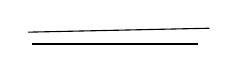
\begin{tikzpicture}\draw (0,0.05)--(2.3,0.10);\draw (0.05,-0.10)--(2.15,-0.10);\end{tikzpicture}}

Supposons qu'on ait une catégorie de Deuring \deleted{\unsure{stricte}} sur $A$ \deleted{anneau, tel que de Dedekind,} \inserted{normal, avec $O$ \deleted{\unsure{de rang}} \unsure{fin.} sur $A$ sans torsion et $O_K$ azumaya sur $K$.}
$U\subset S$ le plus grand ouvert sur lequel les $O=\uline{\operatorname{End}}(X)$ (un, tous, c'est kif-kif) soient d'Azumaya. Donc $C$ définit une gerbe \inserted{$\mathcal G_U$} de lien $G_m$ sur $U$, dont la classe dans $\operatorname{Br}(U)$ est tuée par $n$, \inserted{par le ``rang'' de $C$.} et $C\otimes_A\underset{A'}{\uline{\Gamma(U)}}$ se récupère par cette gerbe $\mathcal G_U$, à équivalence canonique (définie à isom uniques) près, \deleted{comme} la catégorie des repr. de cette
\mspage{20}

\scanpage{22}

 gerbe est alors une \inserted{\unsure{Gr-}}catégorie $A'$-linéaire, canoniquement déterminée.

\deleted{Supposons que \deleted{tt $X\in$} \inserted{pour} tout $X\in\operatorname{Ob}C$, et considérons $O=\operatorname{End}(X)$, et
\[
N_{\mathrm{red}}:\unsure{k}\ O^*\longrightarrow A^*
\]}

Nous désirons, sous certaines conditions, en définir un objet inversible canonique, en établissant un système transitif d'isomorphismes entre les $\det(X_{A'})$ $(X\in\operatorname{Ob}C)$. Pour ceci il suffit de définir un isom canonique
\[
(\alpha)\qquad \det P\simeq A
\]
pour tt. module à droite inv. $P$ sur un $O=\operatorname{End}(X)$ $(X\in\operatorname{Ob}C)$, fonctoriel en $P$ (ce qui suppose que
\[
N_{\mathrm{red}}:O'^*\longrightarrow A^*\quad\text{est à valeurs dans }1\}
\]
$O'$ étant le commutant de $O$ dans $P$ ....) et multiplicatif si $\unsure{{}_{O''}Q_{O'}P_O}\,\unsure{\otimes}$
\[
N_{\mathrm{red}}(Q\otimes_{O'}P,O)\simeq N_{\mathrm{red}}(Q,O')\otimes N_{\mathrm{red}}(P,O)
\]
doit être compatible avec les isom \unsure{ass.}. Cela marche si on suppose
\margin{[posant $\Phi=N_{\mathrm{red}}(E^*)\subset K^*$, où $O=\operatorname{End}(X)$, $E=O\otimes_A K$]}
\[
\left\{\begin{array}{l}
\operatorname{Pic}(A)=0\\
\deleted{N_{\mathrm{red}}(E^*)\cap N_{\mathrm{red}}(O)}\\
\Phi\cap A^*=\{1\},\quad \Phi.A^*=K^*
\end{array}\right.
\]
Ces conditions sont vérifiées \deleted{\unsure{pour si} $A=\deleted{\unsure{\mathbf Q}}\inserted{\mathbf Z}$, \illegible{1}} \deleted{\unsure{corps de nb. tot. réel}}, si $A=\mathbf Z$, $E_K(=E_{\mathbf R})$ \unsure{pas décomposé} sur $\mathbf R$. Donc dans ce cas, on a un objet inv. canonique de degré $n$ de $\operatorname{Rep}(\mathcal G_{A'})$, de sorte que le lien \unsure{structural} de la gerbe $\mathcal G_{A'}$

\mspage{21}

\scanpage{23}

se trouve de façon naturelle réduit à $\mu_n$.

On prend maintenant
\[
\begin{gathered}
C=\text{catégorie des courbes elliptiques de}\\
\text{Hasse nul sur corps alg. clos $k$ de car $p$}
\end{gathered}
\]
D'après Deuring, c'est une catégorie de Deuring \inserted{stricte sur $\mathbf Z$}, \deleted{dont} correspondant à la classe d'isomorphie des corps gauches de degré $4$ (corps de quaternions) sur $\mathbf Q$ \deleted{dont} qui \unsure{splitte} en ttes les places sauf $p$ et $\infty$ (il est donc d'ordre $2$ dans $\operatorname{Br}(\mathbf Q)$).

On tire donc, canoniquement en \deleted{\unsure{la}} termes de \deleted{\unsure{G}}\inserted{$C$} [\deleted{la donnée} \inserted{ou de} d'un tel corps sur $\mathbf Q$, une gerbe $\mathcal G$ sur $\operatorname{Spec}\mathbf Z[\frac1p]$ de \deleted{groupe} \inserted{lien} $\mu_{\unsure{2|n}}$ [$\simeq$ Gerbe $\widehat{\mathcal G}$ du \unsure{type|lien} $G_m$, $+$ représentation \inserted{inversible, $T$,} de ce dernier, de rang $2$]. On trouve de plus, si
\[
A'=\prod_{\ell\ne p,\infty}\mathbf Z_\ell,
\]
une \deleted{représentation de $\unsure{\mathcal G}_{A'}$ de rang $2$, degré $1$, soit $E$, (\unsure{donc un isom} \unsure{avec une repr.} de $\mathcal G_{A'}$ de rang $2$, degré $\unsure{1_T|1}$), avec
\[
\det E\simeq T
\]}
\inserted{banalisation de $C_{A'}$, i.e.}
\inserted{i.e. une trivialisation de $\widehat{\mathcal G}_{A'}$, $\varphi$, \deleted{\unsure{ou}}}
\margin{\fbox{i.e. foncteur fibre $\varphi$ de $\operatorname{Rep}(\widehat{\mathcal G}_{A'})$ sur $A'$}}
\inserted{muni} d'un isom
\[
\deleted{\unsure{\varphi E}}\qquad
\varphi(T)\simeq A'(1)\left(\overset{\mathrm{def}}=\prod_{\ell\ne p,\infty}\mathbf Z_\ell(1)\right)
\]
\deleted{\unsure{donc} Cela fait donc}
En d'autres termes, si $\mathcal H_{A'}$ est la gerbe des racines carrées de $A'(1)$, qui est une gerbe sous $\mu_{2,A'}$, on a un isomorphisme canonique de

\mspage{22}

\scanpage{24}

\[
\mathcal G_{A'}\simeq\mathcal H_{A'}
\]
Comme invariant ($C$ \unsure{donc} $\mathcal G_{A'}$ \inserted{de $\mathcal G_{A'}$} étant ici fixée) on trouve que cette donnée \inserted{à isom près} représente un point d'un \uuline{torseur} sur
\[
H^1(A',\mu_2)\simeq\prod_{\ell\ne p,\infty}\underbrace{\mathbf Z_\ell^*/\mathbf Z_\ell^{*2}}_{\begin{gathered}\simeq\mathbf Z/2\mathbf Z\text{ si }\ell\ne2\\\simeq\mathbf Z/2\mathbf Z\times\mathbf Z/2\mathbf Z\text{ si }\ell=2\end{gathered}}
\]
\deleted{\[
\unsure{H^2(\mathbf Q\to A',\mu_2)\simeq\operatorname{Coker}(}
\]}
\margin{\uline{NB} il n'y a absolument pas de façon naturelle de choisir une origine \inserted{de façon ``\unsure{abstraite}''} \deleted{\unsure{voir dans cohomologie} \unsure{par des classes} \unsure{dans} $\unsure{\mu_\ell}$ mod $(\mathbf Z/\ell\mathbf Z)^{*2}$ $(\ell\ne2)$ $\unsure{\mu_8}$ mod $(\mathbf Z/8\mathbf Z)^{*2}$}}

Si on tient compte du fait que la gerbe $\mathcal G_{A'}$ est déterminée seulement à équivalence (non unique près), le choix d'une \unsure{classe d'isomorphie d'équivalence permet} \unsure{diffère} donc d'une classe de
\[
H^1(\underbrace{\mathbf Z[\tfrac1p]}_{A'},\mu_2)\simeq\mathbf Z/2\mathbf Z\times\mathbf Z/2\mathbf Z
\]
(\unsure{l'élt} \deleted{un él de $\mathbf Z/2\mathbf Z$} \inserted{$(1,0)$ resp. $(0,1)$} correspond au rev. de groupe $\mu_2$ obtenu par $\sqrt[2]{p}$ \inserted{resp. $\sqrt[2]{-1}$}) on trouve un invariant \deleted{dans} dans un quotient
\[
\Pi/\rho(\mathbf Z/2\mathbf Z),
\]
où $\Pi$ est le torseur sur $H^1(A',\mu_2)=\prod_{\ell\ne p,\infty}\mathbf Z_\ell^*/\mathbf Z_\ell^{*2}$ des trivialisations de $\mathcal H_{A'}$, et
\[
\rho:H^1(\mathbf Z[\tfrac1p],\mu_2)\simeq(\mathbf Z/2\mathbf Z)\inserted{\times\mathbf Z/2\mathbf Z}\longrightarrow H^1(A',\mu_2)
\]
est l'hom naturel, défini par la condition
\[
\rho(1,0)_\ell\inserted{\text{(resp. }\rho(0,1)_\ell\text{)}}=
\begin{cases}
0&\text{si }p\inserted{\text{(resp. }-1\text{)}}\text{ un carré dans }\mathbf Z_\ell^*\quad(\overset{\inserted{\text{si }\ell\ne2}}{\Longleftrightarrow}p\text{ carré dans }(\mathbf Z/\ell\mathbf Z)^*\text{) si }\deleted{\ell\ne2)}\\
1&\text{sinon}
\end{cases}
\]
\margin{on peut éliminer ce groupe $\mathbf Z/2\mathbf Z\times\mathbf Z/2\mathbf Z$ grâce à la donnée de la structure \unsure{suppl.} \unsure{a)} polarisation à l'$\infty$ b) ``cristalline'' en $p$}
\figure{\begin{tikzpicture}[x=1cm,y=1cm]\draw (0.04,0.34) -- (0.08,0.17);\draw (0,0.20) .. controls (-0.03,0.10) and (0.06,0.03) .. (0.10,0);\end{tikzpicture}}

\mspage{23}

\scanpage{26}

\uline{Cat. de Deuring sur} $A$

C'est une catégorie pré-additive, $\unsure{A|O}$-linéaire telle que
\diagram{\begin{tikzcd}[row sep=large]
{\exists\ A\text{-algèbre }O,\ \text{avec } C\underset{\text{équiv. $A$-linéaire}}{\simeq}\underbrace{\mathbb P(O/A)}_{\substack{\text{modules à droite}\\\text{sur $O$ loc. libres de}\\\text{rang $1$ sur $\operatorname{Spec}A$}}}} \arrow[d,Leftrightarrow] \\
{\begin{gathered}\exists X_0\in\operatorname{Ob}C\quad\text{t. q.}\quad\text{a) pour }\forall P\in\operatorname{Ob}\mathbb P(O/A),\quad\text{où }O=\operatorname{End}_C(X_0),\\P\otimes_O X_0\,\unsure{\otimes}\ \text{existe}\qquad\text{b) }P\longmapsto P\otimes_O X_0\quad\text{une équivalence de catégories}\end{gathered}} \arrow[d,Leftrightarrow] \\
{\forall X_0\in\operatorname{Ob}C,\quad\text{on a}\quad\text{a) b)}}
\end{tikzcd}}

\uline{NB} A équiv. (non unique) près, $C$ est donc défini par une algèbre $O$. Pour que $O$, $O'$ définissent des $C$ équivalentes, il f. et s. qu'il existe $P\in\mathbb P(O/A)$, avec $O'\simeq\operatorname{End}(P)$, i.e. que $O'$ soit obtenu en ``tordant par \unsure{autom. intérieurs} par un $P\in\mathbb P(O/A)$''. Si $O$ est commutatif (cas intéressant !) on trouve que $O\simeq O'$.

\deleted{\uline{\unsure{Précisions}}},
Soient $C$, $C'$ deux catégories \inserted{$A$-lin. resp $A'$-lin.}, avec $A\overset{\alpha}{\mathbin{-}}A'$ donné. Supposons $C$ de Deuring. Un foncteur $F:C\mathbin{-}C'\deleted{\unsure{A\to A'}}$ est dit \uline{admissible} \inserted{(\unsure{pour} $\alpha$)} s'il est $A$-linéaire, et s'il \unsure{commute} à l'opération $P\otimes_O X$ pour $X\in\operatorname{Ob}C$, $O=\operatorname{End}_C(X)$, $P\in\mathbb P(O/A)$. Il suffit

\mspage{25}

\scanpage{28}

de \unsure{l'image par|l'image près} $\simeq X$, et pour $X$ fixé, la \deleted{\unsure{donnée de}} catégorie \unsure{des} ces foncteurs est équivalente à la catégorie des couples $(X',\unsure{u|\alpha})$ où
\[
\begin{gathered}
X'\text{ est un objet de }C'\\
u:O=\operatorname{End}(X)\longrightarrow O'=\operatorname{End}(X')\quad\text{un hom comp. avec }A\to A'
\end{gathered}
\]
\uline{Hyp}\quad $\forall P\in\operatorname{Ob}\mathbb P(O/A)$, \deleted{$\unsure{P\otimes}$} posant $P'=P\otimes_O O'\in\mathbb P(O'/A')$ le produit tensoriel $P'\otimes_{O'}X'$ existe

[\uline{NB} la Hyp est superflue si p. ex. $C'$ est elle-même une catégorie de Deuring]

\deleted{\unsure{Corollaire}}
Catégorie $C_{A'}$ (catégorie de Deuring sur $A'$, \unsure{correspond} : solution d'un pb universel)
\[
\operatorname{Hom\,ad}_{A\unsure{\longmapsto|\longrightarrow}A'}(C,C')\simeq\operatorname{Hom.ad}_{A'}(C_{A'},C')\ ]
\]

\deleted{Si $C$, $C'$ sont de Deuring les deux}, Pour que $C_{A'}\mathbin{-}C'$ soit une équivalence, il faut que $C'$ soit de Deuring aussi, et que $O\otimes_A A'\mathbin{-}O'$ soit un isomorphisme.

Le Gr-catégorie des autoéquivalences de $C$ est \inserted{$\simeq$} la catégorie des bitorseurs $P$ sous $O$, $O$, loc. sur $A$ inv. pour les deux structures, avec le produit tensoriel évident. Si $A=A'$,

\mspage{27}

\scanpage{30}

la catégorie des équivalences de $C$ avec $C'$ ($C'$ étant de Deuring) est une \unsure{Trs-|Tors-}catégorie sous le Gr-catégorie précédente.

\uline{Ex 1} Soit $A$ anneau de Dedekind, \inserted{corps fractions $K$.} Pour \unsure{tt} \deleted{Algèbre} \unsure{classe|classes} d'isomorphie d'algèbres \inserted{finie} ass. semi-simples $E$ sur $K$, on obtient une classe d'équivalences de catégories de Deuring : les catégories
\[
\mathbb P(O/A)\simeq\mathbb P(O/\text{centre de }O)
\]
définies par les \uline{ordres maximaux} de $E$ : \inserted{catégorie de Deuring de type $E$.} \unsure{Construction} commute à tte extension de base $A\mathbin{-}A'$, avec $A'$ un corps ou un anneau de Dedekind à ext. résiduelles ttes triviales (ex. : localisations henséliennes, complétions --- mais \uuline{pas} localisations étales !!).

\margin{La catégorie des autoéquivalences d'une telle $C$ a comme $\pi_1$ le groupe $Z^*$, où $Z$ est la clôture entière de $A$ dans le centre de $E$. (Donc si $E$ central sur $\unsure{A|K}$, $\pi_1=A^*$)}

Si $A$ est local, $E$ \unsure{centrale|simple} de centre $K$, alors la \inserted{Gr-}catégorie \deleted{\unsure{End|Aut}} des autoéquivalences d'une $C$ de Deuring de type $E$ est un $\pi_0=1$ (tt bimodule sur $O$ biinvble des deux côtés est trivial). \deleted{Donc la catégorie} \inserted{Mais} il reste le $\pi_1=A^*$.

\mspage{29}

\scanpage{32}
\uline{Ex. 2} Soit $C$ comme dans Ex. 1 et soit $\unsure{\mathcal P|\mathcal D}$ une catégorie de Deuring reliée à $A$. Un \uline{foncteur norme} de $C$ à $\unsure{\mathcal P|\mathcal D}$ est un couple $(\nu,\alpha)$, où
\[
\nu:C\longrightarrow D\qquad\text{un foncteur (en général pas additif!)}
\]
\[
\alpha=(\alpha_{X,P}):\nu(P\otimes_O X)\xrightarrow{\sim}
\underbrace{\operatorname{Nr}_{O/A}}_{\text{norme réduite}}(P)\otimes_A\nu(X)
\]
un système d'isomorphismes, satisfaisant les conditions de transitivité, et fonctorialité en $P,X\ldots$.

\margin{\unsure{Généraliser} au cas où $\unsure{\mathcal P|D}$ n'est pas néc. de Deuring, mais seulement \inserted{$A$-lin.} \unsure{que les} $\operatorname{Nr}_{O/A}(P)\otimes_A Y$ $(Y\in\operatorname{Ob}\unsure{\mathcal P|D})$ existent.
\figure{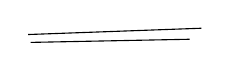
\begin{tikzpicture}[x=1cm,y=1cm]\draw (0,0)--(2.2,.08);\draw (.03,-.10)--(2.05,-.06);\end{tikzpicture}}
Montrer qu'il y a une $D$ universelle recevant un foncteur norme, \unsure{qu'on écrira} $V_A(C)$. \deleted{$\unsure{N_{A/K}(C)|N_A(C)}$} Noter que $V_A(C)$ commute aux chgts de base du type envisagé en Ex. 1 \deleted{\unsure{ce qui est}}.}

\deleted{Pour} \unsure{Si} $X$ fixé dans $\operatorname{Ob}C$, la cat. des foncteurs \deleted{déterminants}\inserted{normes} est \inserted{can.} équiv. \deleted{can.} à celle des objets $T_0$ de $\unsure{D}$, en définissant $\nu$ par
\[
\nu(P\otimes_O X)\simeq\operatorname{Nr}_{O/A}(P)\otimes T_0.
\]
\diagram{\begin{tikzcd}
\deleted{C}\arrow[r,phantom,"{\deleted{(\nu,\alpha)}}","{\deleted{\longrightarrow}}"{description}]&\deleted{D}
\end{tikzcd}}
Supposons maintenant qu'on ait un isom fonctoriel en $P\in\mathbb P(O/A)$
\[
\operatorname{Nr}_{O/A}(P)\simeq A
\]
\margin{avec conditions de transitivité\ldots \unsure{compatibilités}}
\diagram{\begin{tikzcd}
\deleted{A}\arrow[r,phantom,"{\deleted{\longrightarrow}}"{description}]&\deleted{\unsure{A\prime|A}}
\end{tikzcd}}
\margin{Noter qu'alors la catégorie $V_A(C)$ est munie d'une section canonique $\tau$ et $\nu_C$ est \unsure{c\textsuperscript{te} v.l.} $\tau$.}
Soit $A'\mathbin{-}A$ un chgt de base du type envisagé dans ex. 1, et considérons \deleted{$\unsure{E}$} sur $A'$ des catégories de Deuring $C',D'$, et un hom norme $(\nu,\alpha):C'\mathbin{-}D'$. Soit enfin $\varphi:C\mathbin{-}C'$ un foncteur admissible.
\diagram{\begin{tikzcd}
C\arrow[r,"\varphi"]&C'\arrow[r,"\nu"]&D'\\
A&A'&
\end{tikzcd}}
Alors \deleted{\unsure{p}} on a un objet can. $T_\varphi$ de $D'$, et un isom $\nu(\varphi(X))\simeq T_\varphi$.
\mspage{31}
